
\subsection{Изучение характеристик голограммы точечного источника}

    В работе предлагается рассчитать расстояние от голограммы до точечного источника, 
    который использовался при её создании:
    \begin{itemize}
        \item по результатам измерения радиусов голографических колец,
              спроецированных на экран при помощи короткофокусной линзы
        \item по результатам измерения параметров проекционной установки, 
              в которой голограмма используется как фокусирующая линза, 
              а объектом служит предметная шкала.
    \end{itemize}

    \subsubsection*{Определение цены деления предметной шкалы}

        Устанавливаем кассету с транспарантами вблизи лазера. Освещаем лучом лазера шкалу и 
        получаем на удалённом экране дифракционную картину, созданную крестообразной шкалой.

        По результатам измерений $\Delta x = (0.55 \pm 0.01)$ см, $L = (118.5 \pm 0.2)$ см.
        $\lambda$ известно и равно $532$ нм. Отсюда из формулы для дифракции Фраунгофера
        находим цену деления: $D = \frac{\lambda \cdot L}{\Delta x} = (115 \pm 2)$ мкм.

        Определим цену деления той же шкалы, используя линзу с фокусным расстоянием
        $F = 40$ мм, $a = (4.6 \pm 0.1)$ см, $b = (113.5 \pm 0.1)$ см. Находим
        $\Gamma = \frac{b}{a} = (26.7 \pm 0.5)$. По результатам измерений
        $D' = (0.26 \pm 0.02)$ см. Таким образом $D = \frac{D'}{\Gamma} = (97 \pm 17)$ мкм.

        По размерам погрешностей видно, что первый способ точнее.

    \subsubsection*{Определение расстояние от голограммы до точечного источника}

        Получили на экране контрастное изображение колец. Результат измерения их радиусов:

        \import{src/}{table.tex}

        \begin{figure}[h!]
            \center{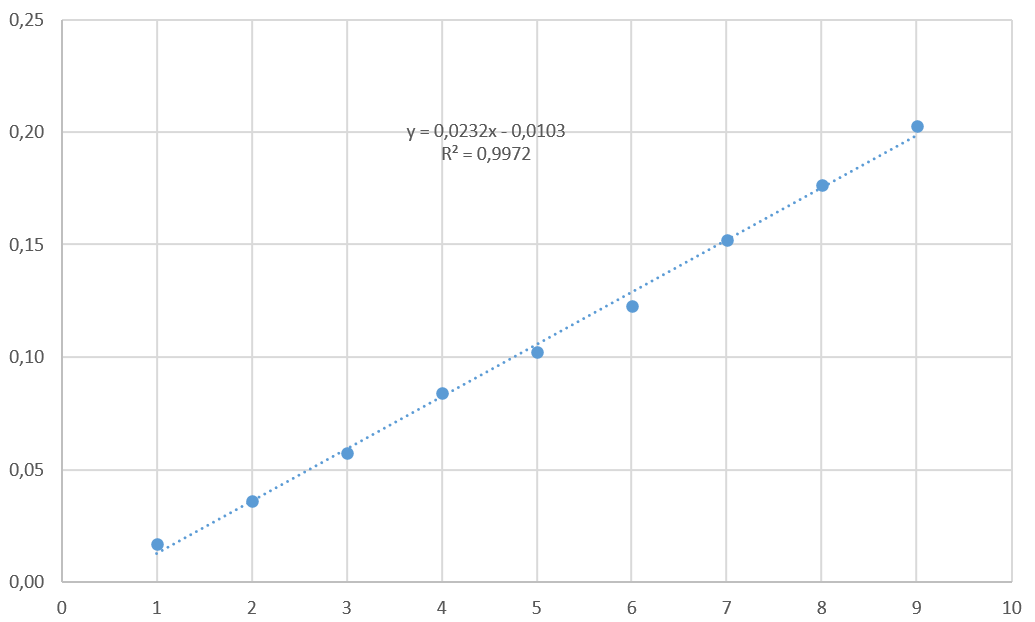
\includegraphics[width=0.9\linewidth]{graph.png}}
            \caption{График зависимости $r^2$ от $m$}
        \end{figure}

        Из формулы 
        \\
        $$
        r = \sqrt{m \lambda d}
        $$
        \\
        следует:
        \\
        $$
        d = \frac{1}{\lambda} \frac{\Delta r^2}{\Delta m}
        $$
        
        Из графика получим, что $\frac{\Delta r^2}{\Delta m} = (2.29 \pm 0.05) 10^{-2} \: мм^2$.
        А следовательно расстояние до точечного источника, использованного при создании 
        голограммы $d = (43 \pm 1)$ мм.

        Перемещая линзу вдоль луча получаем на экране изображения мнимого источника $O_2$
        и действительного $O_3$. Зная фокусное расстояние лизны $F = 4$ см, а также 
        расстояние от лазера до каждого из изображений источников 
        $\rho(\text{Л}, O_2^*) = (2.3 \pm 0.1)$ см,
        $\rho(\text{Л}, O_3^*) = (8.8 \pm 0.1)$ см из формулы тонкой линзы: 
        \\
        $$
        \frac{1}{a} + \frac{1}{b} = \frac{1}{F}
        $$
        \\
        находим $\rho(\text{Л}, O_2) = (-5.4 \pm 0.6)$ см,
        $\rho(\text{Л}, O_3) = (7.3 \pm 0.3)$ см

    \subsubsection*{Изучение фокусирующих свойств голограммы}

        Добиваемся полного разделения пучков света на экране и определяем, какой из них соответствует действительному, какой мнимому изображению. 

        \noindent Установив перед голограммой предметную шкалу, получаем четкое изображение шкалы в пятне, соответствующем действительному изображению.
        
        \noindent Измерьте расстояние между штрихами $ \Delta x $ на экране и расстояние $L$ от экрана до голограммы. Используя эти данные, а также найденную ранее цену деления шкалы $D$, рассчитаем фокусное расстояние голографической линзы.
        
        \[ \Delta x = \frac{(9.5 \pm 0.5) \; мм}{7} = (1.36\pm 0.07) \; мм   ; \quad L = (510 \pm 5) \; мм \]
        \[ F = \dfrac{L}{1+\frac{D}{\Delta x}} = (4.6 \pm 0.1) \; см \]
        
\subsection{Изучение характеристик голограммы объемного предмета}
    \subsubsection*{Изучение мнимого изображения}
        
        \noindent Настроив систему и поместив голограмму в расширенный пучок лазера фотоэмульсией к лазеру находим мнимое изображение предмета. 
        $ \alpha = 32^o \pm 2^o $~--~угол поворота голограммы (угол падения опорного пучка).
        
        Постепенно закрываем голограмму листом бумаги и видим, что изображение почти не меняется, то есть восстанавливается не из полной картины.        
        На мнимом изображении видим линейку, а за ней стержень. На действительном изображении стержень расположен перед линейкой. 
        Оценим расстояние $h$ от линейки до вертикального стержня. Для этого рассмотрим отметку на линейке при разных углах поворота. Для угла $\alpha = 30^o$ при повороте на $\Delta \alpha =  10^o$ стержень соответствует делениям отстоящим на $l = 6$ мм. Тогда: \[h \approx \frac{l \cos \alpha}{\Delta \alpha} = 3 \; cm \]

    \subsection{Изучение действительного изображения}

        Находим действительное изображение, поворачиваем голограмму на $180^o$ вокруг вертикальной оси.
        Угол падения восстанавливающей волны, при которых возникает действительное изображение~--~$30^o$, мнимое изображение~--~$24^o$.
        Снова разворачиваем голограмму эмульсией к лазеру. Перемещаем короткофокусную линзу расширителя вдоль луча, наблюдаем, что при приближении линзы к лазеру изображение действительное увеличивается, мнимое уменьшается.
